\section{Ejercicio}\label{ej:Chap02Ejercicio01}

El aparato de la figura \ref{im:002} se coloca en una habitación cerrada a $\SI{20}{\celsius}$. Una batería de paredes metálicas está conectada a un motor que actúa un agitador sumergido en un líquido contenido en un tanque de paredes rígidas. El motor tiene un rendimiento del $80\%$. Es decir, el $80\%$ del trabajo eléctrico aparece como trabajo en el eje.

El proceso se considera estacionario para todos los elementos componentes. El líquido permanece a una temperatura de $\SI{50}{\celsius}$ y la batería a $\SI{35}{\celsius}$.

Dibujar claramente la frontera y establecer los signos del trabajo $W$ y el calor $Q$ para los siguientes sistemas

\begin{figure}[h]
\centerline{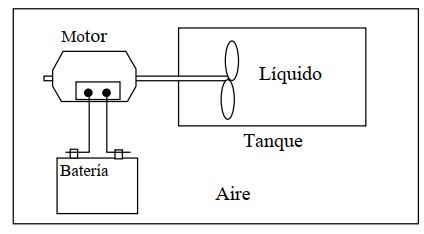
\includegraphics[scale=0.8]{002.jpg}}
\caption{\textit{El dispositivo está en equilibrio mecánico. El pistón se puede deslizar libremente y sin rozamiento.}}
\label{im:002}
\end{figure}

\begin{enumerate}
\item Batería.
\item Motor.
\item Agitador y líquido.
\item Líquido.
\item Aire.
\item Batería y aire.
\item Motor y agitador.
\item Líquido, tanque y aire.
\item Tanque.
\end{enumerate}